\section{Overview}
%Trong những năm gần đây, ta đã chứng kiến sự phổ biến và sức mạnh của các mô hình học sâu (Deep Learning models) trong nhiều loại ứng dụng khác nhau trong đời sống thực tiễn. Sức mạnh của các mô hình học sâu này được tăng cường theo từng ngày. Sự phát triển mạnh mẽ về tài nguyên tính toán cho phép các mô hình ngày càng trở nên lớn hơn và phức tạp hơn về mặt kích thước như là số lượng tham số và độ sâu. Ngoài ra, việc đầu tư mạnh mẽ vào nghiên cứu đã khuyến khích phát triển nên các kiến trúc đạt hiệu suất cao hơn nhưng cũng làm chúng trở nên phức tạp hơn với những người sử dụng.

In recent years, we have witnessed the rising popularity and effectiveness of deep learning models across diverse real-world applications. The power of these deep learning models has been amplified as the massive growth in computational resources allows models to become increasingly larger and more complex in dimensions, as evidence in the growing number of parameters and depth. Moreover, substantial investment in research has encouraged the development of more efficient architectures but has also made them more complex for users.

%Trong nhiều lĩnh vực thực tế, các hệ thống trí tuệ nhân tạo có thể được sử dụng để đưa ra các quyết định quan trọng có thể ảnh hưởng đến tính mạng của con người như y tế, an ninh hay tự động hóa. Chính vì thế, khi ứng dụng trí tuệ nhân tạo để giải quyết vấn đề, việc hiểu rõ lý do và quy trình mà một mô hình học máy sử dụng để đưa ra quyết định trở nên vô cùng quan trọng.

In some high-stake domains, artificial intelligence systems play a pivotal role in making consequential decisions that can significantly impact human lives, such as in healthcare, security, and automation. However, as deep learning models become more and more complex, we are at risk of being dependent on systems that we do not understand. Delegating the work to the models without seriously questioning the reasons for their decisions can be dangerous. Because in the end, deep learning systems can be unfair because they learn from data generated by humans, which inherently contain biases. Hence, comprehending the reasoning and decision-making processes of deep learning models is vital.

%Trí tuệ nhân tạo có khả năng giải thích (eXplainable Artificial Intelligence) dần nổi lên như là một giải pháp cho các vấn đề trên. Trong lĩnh vực thị giác máy tính nói riêng, Saliency là hướng tiếp cận mà trong đó việc giải thích tập trung vào trực quan hoá mức độ ảnh hưởng của những vùng/điểm (pixel) trên ảnh lên kết quả dự đoán của một mô hình bằng thứ gọi là "saliency maps". Việc hiểu mô hình sử dụng những phần nào trên tấm ảnh để dự đoán giúp ta tìm ra những điểm yếu và hạn chế của các mô hình hiện tại cải thiện chúng hoặc phát triển nên các phiên bản mới hơn.

eXplainable Artificial Intelligence (XAI) is an active field that aims to tackle the issue of making complex models more interpretable to users. With the availability of interpretable models, trust and awareness can be gained, especially for high-stake applications. For example, in the medical domain, the COVID-19 pandemic has motivated researchers to address its related challenges and contribute to disease prevention. Several studies have employed deep learning models to tackle computer vision problems such as anomaly detection in endoscopic, X-ray images, etc. With the development of XAI, researchers no longer solely focus on measuring the model performance by metrics, but also its interpretability. This is crucial not only for transparency but also for establishing trust when employing artificial intelligence to address problems \cite{explainableCovidModel}.

In the literature, models that are complex and difficult to interpret are commonly known as ``black boxes''. There are various approaches to making a black box more understandable, such as creating a newer, simpler model that can replicate the behavior of the complex model. Another common method is to provide explanations for individual decisions made by the black box. In computer vision, where images are the input to the black boxes, these explanations are often provided in the form of ``saliency maps'', which assign scores to regions or pixels of the input images, indicating their influence on the model's output. Saliency maps help users to comprehend which parts of an image the model's prediction is based on, making it easier to identify weaknesses and limitations of the model, and thereby improving or creating new versions. Figure \ref{fig:saliencyExample} illustrates an example of using saliency map to explain a model prediction.

\begin{figure}
    \centering
    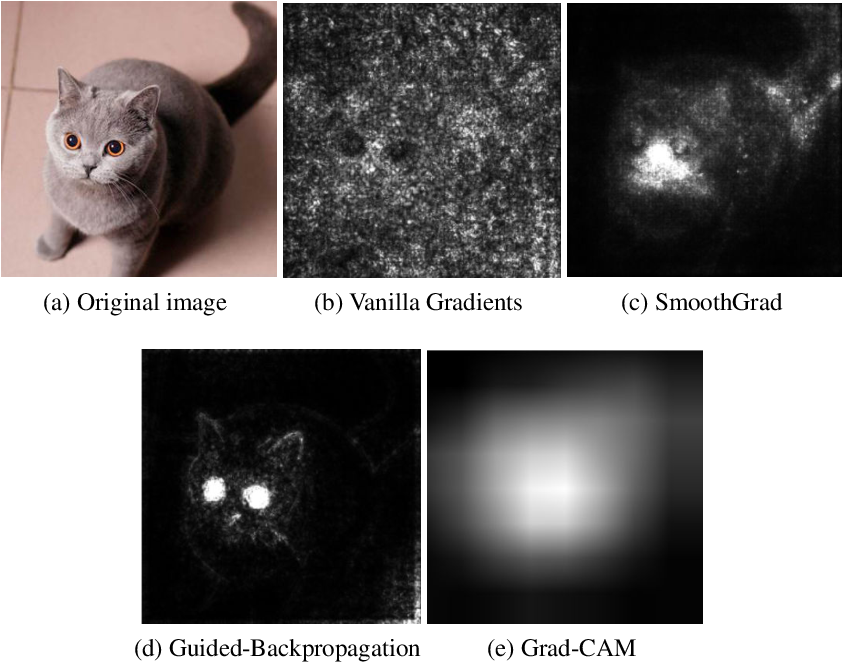
\includegraphics[width=\textwidth]{images/saliency_example.png}
    \caption{Different saliency maps produced by different XAI methods. The bright areas indicate important areas. \cite{crowdsourcing}}
    \label{fig:saliencyExample}
\end{figure}

% Lấy ví dụ trong lĩnh vực y học, COVID-19 vừa qua đã là nguồn động lực to lớn để các nhà nghiên cứu giải quyết các vấn đề xung quanh nó nhằm chung tay góp sức đẩy lùi dịch bệnh. Đã có nhiều nghiên cứu sử dụng các mô hình học sâu để giải quyết các bài toán thị giác máy tính như nhận dạng điểm bất thường trên các ảnh chụp nội soi, XRay,.. Với sự phát triển của XAI, để chứng minh mô hình của mình đạt hiệu quả cao, các nhà nghiên cứu đã không còn chỉ quan tâm đến hiệu suất của mô hình bằng các phép đo (metrics) mà còn phải chứng minh được việc các mô hình có thật sự hoạt động như mong muốn bằng XAI bởi điều này không những ảnh hưởng đến tính minh bạch mà còn là niềm tin khi sử dụng trí tuệ nhân tạo để giải quyết vấn đề \cite{explainableCovidModel}.

% Tuy nhiên, XAI chính nó cũng tồn tại một vấn đề - Sự bất đồng giữa các phương pháp giải thích với nhau trên cùng một mô hình hộp đen (black-box model). Vấn đề này tuy quan trọng, nhưng lại chưa được nghiên cứu rộng rãi nói chung, đặc biệt là y học nói riêng. Nghiên cứu của Krishna và đồng nghiệp \cite{krishna_disagreement_problem} là một trong những nỗ lực đầu tiên nói lên vấn đề không đồng nhất này, bài báo đã chỉ ra sự không nhất quán giữa các mô hình XAI dựa trên tính quan trọng của đặc trưng trên các loại dữ liệu khác nhau như dữ liệu bảng, văn bản và hình ảnh. 
